\chapter{Bayesian Monte Carlo}
Consider the integral
\begin{equation}\label{integralbmc}
Z = \int_{\mathbb{R}^D} f(x) p(x) dx.
\end{equation}
In the following discussion, we drop  $\mathbb{R}^D$ from the integral symbol, for simplicity. If $p(x)$ is a distribution whose sampling is easy, the bottleneck for a simple Monte Carlo method for estimating $Z$ would be the evaluation cost of $f$. If evaluating $f$ is costly then, a naive Monte Carlo method often becomes infeasible. In this section, we present a GP-based method that tries to circumvent this bottleneck. 

\section{GP approximation for the integrand}
In Bayesian Monte Carlo (BMC), or Bayesian quadrature \cite{Ghahramani_2003,O_Hagan_1991} \footnote{The original name Bayesian quadrature describes more accurately the method, however the name Bayesian Monte Carlo will be used in this text. At the literature, both names can be found in roughly equal proportion}, $f$ itself is treated as a random function, and a GP prior $GP(m,k)$ is put on $f$. Therefore, given a set $\mathcal{D} = \{(x_i,f(x_i))\}_{i=1}^N$ of $N$ evaluations, the posterior random function $f_{\mathcal{D}}$ is also distributed according to a GP. In particular, since linear maps of GPs are themselves GPs \cite{Rasmussen06,Hennig_2012}, this implies that the random variable
\begin{equation}\label{bmcrv}
Z_{\mathcal{D}} = \int f_{\mathcal{D}}(x) p(x) dx
\end{equation}
is a Gaussian random variable. Since we can find the mean by 
\begin{equation}\label{evbmc}
\begin{split}
\Ev[Z_{\mathcal{D}}] = \Ev \left[\int f_{\mathcal{D}}(x) p(x) dx \right] = \int \Ev[f_{\mathcal{D}}(x)] p(x) dx,
\end{split}
\end{equation}
and the variance by,
\begin{equation}\label{varbmc}
\begin{split}
\Var(Z_{\mathcal{D}}) & = \Ev[(Z_{\mathcal{D}} - \Ev[Z_{\mathcal{D}}])^2] \\
& = \Ev \left[\left( \int (f_{\mathcal{D}}(x) - \Ev[f_{\mathcal{D}}(x)]) p(x) dx \right)^2 \right] \\
& = \int \int \Ev \left[(f_{\mathcal{D}}(x) - \Ev[f_{\mathcal{D}}(x)]) (f_{\mathcal{D}}(x') - \Ev[f_{\mathcal{D}}(x')]) \right]  p(x) p(x') dx dx' \\
& = \int \int \Cov(f_{\mathcal{D}}(x),f_{\mathcal{D}}(x')) p(x) p(x') dx dx'.
\end{split}
\end{equation}
We have a complete description of the distribution of $Z_\mathcal{D}$. Now, by substituting \eqref{meancovGPR} in \eqref{evbmc} and \eqref{varbmc}, we have 
\begin{equation}\label{evvarbmc2}
\begin{split}
& \Ev[Z_{\mathcal{D}}] = \int m(x) p(x) dx - \mathbf{z}^T K^{-1} (\mathbf{f}-m(\mathbf{x})) \\
& \Var[Z_{\mathcal{D}}] = \Gamma - \mathbf{z}^T K^{-1} \mathbf{z},
\end{split}
\end{equation}
where $\mathbf{z} = (z_1,...,z_N)^T$, with
\begin{equation}\label{zbmcdef}
z_i = \int k(x,x_i) p(x) dx,
\end{equation}
and 
\begin{equation}\label{varcoef}
\Gamma = \int \int k(x,x') p(x) p(x') dx dx'.
\end{equation}
In general, a good estimate of $Z_\mathcal{D}$ is its mean, although if there is an asymmetric loss function associated with estimating $Z_\mathcal{D}$, its variance should be taken in account.

An illustration of the Bayesian Monte Carlo approach to integration is shown in Figure \ref{bmcfig}. There, the distribution is $p(x) = \mathcal{N}(x|0,0.5)$, and $f(x) = -x^2$. The true value of the integral, and BMC estimation are shown. Notice that, in this example, for $|x|>2$ the GP estimate $m_\mathcal{D}(x)$ of $f(x)$ becomes very inaccurate. However, since low probability mass is assigned outside the interval, the BMC estimation is still close to the target.

\begin{figure}
	\centering
	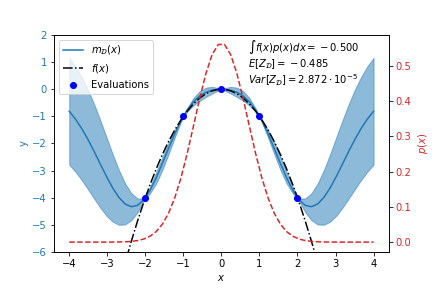
\includegraphics[width=0.7\linewidth]{figs/exbmc.png}
	\caption[Illustration of Bayesian Monte Carlo integration]{\label{bmcfig} Illustration of Bayesian Monte Carlo integration. Here, dash-dot black is $f(x)$, whose value is on the left-axis, while in blue is it's GP mean (dark), and covariance (light), given 5 evaluations (blue circles). In red is $p(x)$, whose value is on the right axis. The true value of the integral, the BMC mean and variance are shown on the top right.}
\end{figure}

\subsection{Philosophical remark}
At first one may find strange to consider $f$ as a random function, in order to give a prior for it. After all, $f$ is a known, fixed function. However, notice that $f$ is only actually known in so far as one can evaluate it, and if evaluations for $f$ are limited, so is the knowledge of it. And by the discussion in Chapter 1, any object the learner has limited knowledge about should be considered a random variable, independent of the fact that the object is actually random or not.

If this philosophical approach is not convincing, maybe it is better to just think of the BMC method as an artificial way to integrate functions, and follow the famous dictum in quantum mechanics: "Shut up and calculate" \cite{Mermin_2004}.


\section{Kernel-distribution combinations}\label{kerneldistributionbmc}
In general, neither \eqref{zbmcdef} nor \eqref{varcoef} are analytically available, just like the original integral \eqref{integralbmc}. However, evaluating the kernel function is in general cheap, so if evaluation of $f$ is expensive, there may be still computational gains in using BMC. For some particular distributions $p(x)$, combined with some suitable kernel choices, \eqref{zbmcdef} nor \eqref{varcoef} does lend analytical solutions, or can be treated in a relatively cheap manner. In the following, $m(x) = 0$ for simplicity, thus omitting the term.

\subsection{SQE kernel with Gaussian distributions}
Assume $p(x) = \mathcal{N}(x|\mu,\Sigma)$, and $k$ is a anisotropic squared exponential kernel, with vertical scale $\theta$ and length scales $l = (l_1,...,l_D)$. Notice then that, by letting $A := \text{diag}(l_1^2,...,l_D^2)$, we have 
\begin{equation} \label{rbfasnormal}
\begin{split}
k(x,x') = \theta \exp \left( -\frac{1}{2} (x - x')^T A^{-1} (x - x') \right) = & \det(2 \pi A) \mathcal{N}(x'|x,A) = \\
& \det(2 \pi A) \mathcal{N}(x|x',A).
\end{split}
\end{equation}
Then, by \eqref{productgaussians}:
\begin{equation} \label{kpexpansion1}
\begin{split}
& k(x,x') \mathcal{N}(x|\mu,\Sigma) = C(x') \mathcal{N}(x|\tilde{\mu}_{x'},\tilde{\Sigma}) \\
& C(x') = \frac{\theta}{\det(I + A^{-1} \Sigma)^{1/2}} \exp \left(-\frac{1}{2}(x' - \mu)^T (A + \Sigma)^{-1}(x' - \mu) \right) \\
& \tilde{\mu}_{x'} = (A^{-1} + \Sigma^{-1})^{-1} (A^{-1} x' + \Sigma^{-1} \mu) \\
& \tilde{\Sigma} = (A^{-1} + \Sigma^{-1})^{-1},
\end{split}
\end{equation}
and
\begin{equation} \label{kpexpansion2}
\begin{split}
& k(x,x') \mathcal{N}(x|\mu,\Sigma) \mathcal{N}(x'|\mu,\Sigma) = \hat{C} \mathcal{N}(x|\tilde{\mu}_{x'},\tilde{\Sigma}) \mathcal{N}(x'|\tilde{\mu}_{x},\tilde{\Sigma}) \\
& \hat{C} = \frac{\theta}{\det(I + 2 A^{-1} \Sigma)^{1/2}}.
\end{split}
\end{equation}
Hence, by substituting \eqref{kpexpansion1} and \eqref{kpexpansion2} into \eqref{zbmcdef} and \eqref{varcoef}, we find 
\begin{equation}\label{termsbmcgaussian}
\begin{split}
& z_i = \frac{\theta}{\det(I + A^{-1} \Sigma)^{1/2}} \exp \left(-\frac{1}{2}(x_i - \mu)^T (A + \Sigma)^{-1}(x_i' - \mu) \right) \\
& \Gamma = \frac{\theta}{\det(I + 2 A^{-1} \Sigma)^{1/2}}.
\end{split}
\end{equation}
Substituting in \eqref{evvarbmc2} we find the desired result:
\begin{equation}\label{evvarbmcgaussian}
\begin{split}
& \Ev[Z_{\mathcal{D}}] = \mathbf{z}^T K^{-1} \mathbf{f} \\
& \Var[Z_{\mathcal{D}}] = \frac{\theta}{\det(I + 2 A^{-1} \Sigma)^{1/2}} - \mathbf{z}^T K^{-1} \mathbf{z} \\
& z_i = \frac{\theta}{\det(I + A^{-1} \Sigma)^{1/2}} \exp \left(-\frac{1}{2}(x_i - \mu)^T (A + \Sigma)^{-1}(x_i' - \mu) \right) \\
& \Gamma = \frac{\theta}{\det(I + 2 A^{-1} \Sigma)^{1/2}}.
\end{split}
\end{equation}

\subsection{Mixture distributions}\label{bmcmixtures}
Consider taking expectations in respect to a mixture distribution
\begin{equation}
 p(x) = \sum_{i=1}^M \alpha_i p_i(x).
\end{equation}
From \eqref{zbmcdef} and \eqref{varcoef}, it is straightforward to see that in this case
\begin{equation}
\begin{split}
 z_i & = \sum_{i=1}^M \alpha_i \int k(x,x_i) p_i(x) dx \\
 \Gamma &= \sum_{i=1}^M \sum_{j=1}^M \alpha_i \alpha_j \int \int k(x,x') p_i(x) p_j(x') dx dx'.
\end{split}
\end{equation}
Then, provided it is possible to calculate the integrals above for each component $p_i(x)$, one can easily use mixture distributions from these coefficients.


An important case is considering mixtures of normal distributions $p(x) = \sum_{j=1}^{M} \alpha_j \mathcal{N}(x|\mu_j,\Sigma_j)$, and the squared-exponential kernel. Then, by substituting in \eqref{zbmcdef} and \eqref{varcoef}, and considering the results for normal distributions in \eqref{termsbmcgaussian}, we find 
\begin{equation}\label{bmcmixgaussians}
\begin{split}
 & z_i = \sum_{j=1}^M \alpha_j z_{i,j} \\ 
 & z_{i,j} = \frac{\theta}{\det(I + A^{-1} \Sigma_j)^{1/2}} \exp \left(-\frac{1}{2}(x_i - \mu_j)^T (A + \Sigma_j)^{-1}(x_i' - \mu_j) \right) \\
 & \Gamma = \sum_{j=1}^M \sum_{m=1}^M \alpha_j \alpha_m \Gamma_{j,m}, \\
 & \Gamma_{j,m} = \frac{\theta}{\det(I + A^{-1} (\Sigma_j+\Sigma_m))^{1/2}} \exp \left(-\frac{1}{2}(\mu_j-\mu_m)^T (A + \Sigma_j + \Sigma_m)^{-1}(\mu_j-\mu_m)\right).
\end{split}
\end{equation}

\subsection{Tensor product kernels and diagonal-covariance Gaussian distributions}\label{tensorprodbmc}
Consider tensor product kernels in $\mathbb{R}^D$ of the form
\begin{equation}
 k(x,x') = \prod_{d=1}^D k_d(x_d,x'_d),
\end{equation}
and a Gaussian distribution $p(x) = \mathcal{N}(x|\mu,\Sigma)$ with diagonal covariance $\Sigma = \text{diag}(\sigma_1^2,\ldots,\sigma_D^{d})$, so that $p(x) = \prod_{d=1}^D \mathcal{N}(x_d|\mu_d,\sigma_d^2)$. Then, 
\begin{equation}\label{prodkernelz}
\begin{split}
 z_i & = \int \prod_{d=1}^D k_d(x_d,x_{i,d}) \prod_{d=1}^D \mathcal{N}(x_d|\mu_d,\sigma_d^2) dx \\
 & = \prod_{d=1}^D \int k_d(x,x_{i,d}) \mathcal{N}(x|\mu_d,\sigma_d^2) dx,
\end{split}
\end{equation}
and 
\begin{equation}\label{prodkernelgamma}
\begin{split}
 \Gamma & = \int \int \prod_{d=1}^D k_d(x_d,x'_d) \prod_{d=1}^D \mathcal{N}(x_d|\mu_d,\sigma_d^2) \prod_{d=1}^D \mathcal{N}(x'_d|\mu_d,\sigma_d^2) dx dx' = \\
 & = \prod_{d=1}^D \int \int k_d(x,x')\mathcal{N}(x|\mu_d,\sigma_d^2)\mathcal{N}(x'|\mu_d,\sigma_d^2) dx dx'.
\end{split}
\end{equation}
Consider each individual component in \eqref{prodkernelz}. Even with none of then being analytically computable, they can easily be approximated using Gauss-Hermite quadrature, that approximates 
\begin{equation}\label{gausshermite}
\int f(x) \mathcal{N}(x|\mu,\sigma^2) dx \approx \frac{1}{\sqrt{\pi}} \sum_{k=1}^K w_k f(\sqrt{2} \sigma x_k + \mu),
\end{equation}
where $x_i$ are the roots of the physicists' Hermite polynomial
\begin{equation}
 H_K(x) = (-1)^N e^{x^2} \frac{d^K}{dx^K} e^{-x^2},
\end{equation}
and $w_k$ are the associated weights
\begin{equation}
 w_k = \frac{2^{K-1} K! \sqrt{\pi}}{K^2 (H_{K-1}(x_k))^2}.
\end{equation}
An analysis of this approximation can be found in \cite{Liu_1994}. It is important to notice that for each $K$, $\{(x_k,w_k)\}_{k=1}^K$ are fixed, unlike standard Monte Carlo methods that would require sampling from $\mathcal{N}(x|\mu,\sigma^2)$. Applying \eqref{gausshermite} to \eqref{prodkernelz}, one finds that
\begin{equation}
 z_i \approx \prod_{d=1}^D \frac{1}{\sqrt{\pi}}\sum_{k=1}^K w_k k_d(\sqrt{2} \sigma_d x_k + \mu_d,x_{i,d}),
\end{equation}
and that
\begin{equation}
\Gamma \approx \prod_{d=1}^D \frac{1}{\pi} \sum_{k,k'=1}^K w_k w_{k'} k_d(\sqrt{2} \sigma_d x_k + \mu_d,\sqrt{2} \sigma_d x_{k'} + \mu_d).
\end{equation}

By the discussion in section \ref{bmcmixtures}, one can easily extend this to mixtures of Gaussians with diagonal covariance. Therefore, one is free to use more flexible kernels than the squared exponential one, provided they are tensor product kernels. The trade-off is that $p(x)$ is a more restrictive distribution, but, as discussed next, this is not an insurmountable restriction. Moreover, the techniques presented in chapters 4 and 5 uses exactly those kinds of distributions as approximations.

\subsection{Importance reweighting for Bayesian Monte Carlo}
One can use the above results for doing integral estimations for general distributions using squared exponential kernels, without Monte Carlo integration of kernels, by an importance re-weighting trick
\begin{equation}
\int f(x) p(x) dx = \int \frac{f(x) p(x)}{q(x)} q(x) dx,
\end{equation}
where $q(x)$ may be either a normal distribution or a mixture of normals. This becomes interesting because since mixtures of normals can approximate continuous densities arbitrarily close as the number of mixtures goes to infinity \cite{Epanechnikov_1969}, thus providing good re-weighting distributions.


\section{Bayesian Monte Carlo for positive integrands}\label{positivebmc}
For many cases the integral we are interested is one arising from marginalization:
\begin{equation}
 p(\mathcal{D}) = \int L(x) p(x) dx = \int p(\mathcal{D}|x) p(x) dx.
\end{equation}
In particular, in this case $L(x)$ must be a positive function. However, applying the BMC method naively can result in rather inaccurate evaluations, due to the fact that in general, GP regression can predict negative means even when all function evaluations are positive. This way, the positivity of the GP mean for $L(x)$ is not guaranteed, resulting in possibly pathological predictions \cite{Ghahramani_2003}.

In \cite{Osborne_2012}, it is proposed to make a GP regression by putting an prior over $\log L(x) \sim GP(m,k)$. However, this means that for predictive distribution in the original space, $L(x|x_{D}) \sim \text{Lognormal}(m_\mathcal{D}(x),k_\mathcal{D}(x,x))$, which results in
\begin{equation}\label{lntranswrong}
 \Ev \left[ \int L(x|x_\mathcal{D}) p(x) dx \right] = 
 \int e^{m_\mathcal{D}(x)+\frac{1}{2}k_\mathcal{D}(x,x)} p(x) dx,
\end{equation}
which is still non-tractable integral, requiring further approximations. It is proposed in \cite{OHagan_1992} a somehow complicated heuristic to circumvent this problem, relying in a number of approximations whose accuracy is questionable, and an inner application of BMC.

In \cite{Gunter_2014}, the transformation used is the square-root transformation, so the prior for GP regression is over $\tilde{L}(x) = \sqrt{2 L(x) - \alpha}$, with $\alpha$ being a small positive scalar, resulting in $L(x|x_\mathcal{D}) = \alpha + \frac{1}{2} \tilde{L}(x|x_\mathcal{D})^2$. However, this way we have $\Ev[L(x|x_\mathcal{D})] = \alpha + \frac{k_\mathcal{D}(x,x)}{2}(1+m_\mathcal{D}(x)^2)$, hence, just like \eqref{lntranswrong}, we can't arrive at a tractable mean. In order to circunvent this, in \cite{Gunter_2014} two approaches are proposed. The first is a linearization of $\alpha + \frac{1}{2} \tilde{L}(x|x_\mathcal{D})^2$ around $m_\mathcal{D}(x)$, resulting in 
\begin{equation}
 L(x|x_\mathcal{D}) \approx L^{\mathcal{L}}(x|x_\mathcal{D}) = \alpha - \frac{1}{2} m_\mathcal{D}(x)^2 + m_\mathcal{D}(x) \tilde{L}(x),
\end{equation}
which, since it is a affine transformation of $\tilde{L}(x)$, results an approximate GP distribution for $L(\cdot|x_\mathcal{D})$:
\begin{equation}\label{sqlinearization}
\begin{split}
 & L^{\mathcal{L}}(\cdot|x_\mathcal{D}) \sim GP(m_\mathcal{D}^\mathcal{L}(x),k_\mathcal{D}^\mathcal{L}(x)) \\
 & m_\mathcal{D}^\mathcal{L}(x) = \alpha + \frac{1}{2} m_\mathcal{D}(x) \\
 & k_\mathcal{D}^\mathcal{L}(x,x') = m_\mathcal{D}(x) k_\mathcal{D}(x,x') m_\mathcal{D}(x).
\end{split}
\end{equation}
The second proposal is to approximate $L(\cdot|x_\mathcal{D})$ by a random GP-distributed function $L^\mathcal{M}(\cdot|x_\mathcal{D}) = GP(m^\mathcal{M}_\mathcal{D},k^\mathcal{M}_\mathcal{D})$, where $m^\mathcal{M}_\mathcal{D}(x)$ and $k^\mathcal{M}_\mathcal{D}(x)$ are chosen so that $L^\mathcal{M}(\cdot|x_\mathcal{D})$ is moment-matched with $L(\cdot|x_\mathcal{D})$, that is,
 $m^\mathcal{M}_\mathcal{D}(x) = \Ev[L(x|x_\mathcal{D})]$ and $k^\mathcal{M}_\mathcal{D}(x,x') = \Cov(L(x|x_\mathcal{D}),L(x'|x_\mathcal{D}))$. This results in the approximation
 \begin{equation}\label{sqmomentmatched}
  \begin{split}
  & L^{\mathcal{M}}(\cdot|x_\mathcal{D}) \sim GP(m_\mathcal{D}^\mathcal{M}(x),k_\mathcal{D}^\mathcal{M}(x)) \\
  & m_\mathcal{D}^\mathcal{M}(x) = \alpha + \frac{1}{2} (m_\mathcal{D}(x) + k_\mathcal{D}(x,x)) \\
  & k_\mathcal{D}^\mathcal{M}(x,x') = \frac{1}{2} k_\mathcal{D}(x,x')^2 + m_\mathcal{D}(x) k_\mathcal{D}(x,x') m_\mathcal{D}(x).
  \end{split}
 \end{equation}
In particular, both approaches results in tractable integrals for gaussian distributions and SQE kernels.

The idea of moment-matching is extended to a general setting in \cite{Chai_2019}, where it is considered the integral \eqref{integralbmc}, where $f$ is now a function from $\mathbb{R}^D$ to a strict subset $\mathcal{Y}$ of $\mathbb{R}$. In the case presented previously, $\mathcal{Y} = (0,\infty)$, while another important case is $\mathcal{Y} = (0,1)$. Considering an bijective map $\epsilon : \mathbb{R} \to \mathcal{Y}$, it is placed a GP prior $GP(m,k)$ over $g = \epsilon^{-1} \circ f$. Then, the posterior distribution for $f(\cdot|x_\mathcal{D}$ is approximated by a moment-matched GP with mean
$m^\mathcal{M}_\mathcal{D}(x) = \Ev[\epsilon(g(x|x_\mathcal{D}))]$ and $k^\mathcal{M}_\mathcal{D}(x,x') = 
\Cov(\epsilon(g(x|x_\mathcal{D})),\epsilon(g(x'|x_\mathcal{D})))$. In particular, for $\epsilon^{-1}(x) = \log(x)$, the same warping considered in \cite{Osborne_2012}, the moment matched mean and covariance becomes 
\begin{equation}\label{logmomentmatched}
\begin{split}
 & m^\mathcal{M}_\mathcal{D}(x) = e^{m_\mathcal{D}(x) + \frac{1}{2}k_\mathcal{D}(x,x)}\\
 & k^\mathcal{M}_\mathcal{D}(x,x') =e^{m_\mathcal{D}(x) + \frac{1}{2}k_\mathcal{D}(x,x)} e^{m_\mathcal{D}(x') + \frac{1}{2}k_\mathcal{D}(x',x')} \left(e^{k_\mathcal{D}(x,x')}-1\right).
\end{split}
\end{equation}

However, when integrated this GP does not result in a integrable mean or variance. One further proposal of \cite{Chai_2019} is to do a Taylor expansion of $m^\mathcal{M}_\mathcal{D}(x)$, 
\begin{equation}\label{taylormomentmatched}
 m^\mathcal{M}_\mathcal{D}(x) \approx 1 + m_\mathcal{D}(x) + \frac{1}{2} k_\mathcal{D}(x,x) + \frac{1}{2}\left(m_\mathcal{D}(x) + \frac{1}{2} k_\mathcal{D}(x,x)\right)^2 + \ldots,
\end{equation}
and of $k^\mathcal{M}_\mathcal{D}(x,x')$,
\begin{equation}
\begin{split}
 k^\mathcal{M}_\mathcal{D}(x,x')  \approx 1 & + k_\mathcal{D}(x,x') + \frac{1}{2} k_\mathcal{D}(x,x')^2 \\ & +
 k_\mathcal{D}(x,x') \left(m_\mathcal{D}(x) + \frac{1}{2} k_\mathcal{D}(x,x) + m_\mathcal{D}(x') + \frac{1}{2} k_\mathcal{D}(x',x')\right)^2 + \ldots\end{split},
\end{equation}
which, depending on the mean function and kernel function (for instance, zero mean and SQE kernel), is integrable when truncated \cite{Chai_2019}.

The use of function warping raises a question on how to choose the GP hyperparameters. In \cite{Chai_2019}, it is argued that for the moment-matched procedure, one should choose the hyperparameters considering the approximated GP distribution for $f$,  $GP(m^\mathcal{M},k^\mathcal{M}(x,x'))$ and the data $(\mathbf{x},f(\mathbf{x}))$, as opposed to the exact GP distribution for $g$, where it is considered $GP(m,k)$ and the data $(\mathbf{x},g(\mathbf{x}))$. The authors of \cite{Chai_2019} call the first approach \textit{$f$-space} optimization, and the second one \textit{$g$-space} optimization, and it is argued that empirically, $f$-space optimization results in better integral estimations for their test cases. \footnote{Tests with $f$-space optimization in this work weren't successful.}

\section{Choosing evaluation points}

The integral estimate variance $\Var[Z_{\mathcal{D}}]$ yields a natural metric for choosing a set of evaluation points $X_\mathcal{D} = \{x_1,...,x_N\}$. Namely, since $\Var[Z_\mathcal{D}]$ does not depend on the evaluation values $\{f(x_1),\ldots,f(x_N)\}$, one can, given a budget of $N$ evaluations, minimize the function $\alpha_{\text{OBQ}}:\mathbb{R}^{dN} \to \mathbb{R}$ given by
\begin{equation}\label{optimal_bmc}
\alpha_{\text{OBQ}}(X_\mathcal{D}) =  \Var[Z_{\mathcal{D}}](X_\mathcal{D}) = \Gamma(X_\mathcal{D}) - \mathbf{z}(X_\mathcal{D})^T K(X_\mathcal{D})^{-1} \mathbf{z}(X_\mathcal{D})
\end{equation}
However, the evaluation of this function has a $\mathcal{O}(N^3)$ cost, due to the need for matrix inversion, is not necessarily convex, and is defined on a very high dimensional space, so its minimization will be feasible only in specific cases. An easier way would be to take a greedy approach, that is, given $X_{\mathcal{D}_{m}} = \{x_1,...,x_m\}$ previously chosen evaluation points, with $m < n$, we choose $x_{m+1}$ such that the variance of $Z_{\mathcal{D}_m \cup \{x_{m+1},f(x_{m+1})\}}$ is minimized, that is, we are looking to minimize the objective function 
\begin{equation}
\alpha^m_{\text{SBQ}}(x_{m+1}) = \alpha^m_\text{OBQ}(x_{m+1};x_1,\ldots,x_m)
\end{equation}

\begin{equation}\label{sequential_bmc}
\alpha^m_{SBQ} : \mathbb{R}^d \to \mathbb{R} , \quad x_{m+1} \to \Var[Z_{\mathcal{D}^m \cup \{x_{m+1},f(x_{m+1})\}}](x_{m+1}),
\end{equation}
This algorithm is referred as Sequential Bayesian Quadrature (SBQ) in \cite{Briol_2015}, while in the same work the first objective is referred as Optimal Bayesian Quadrature (OBQ). Notice that the kernel matrix Cholesky decomposition can be updated in $\mathcal{O}(N^2)$ by the discussion in Section \ref{onlinelearningsection}, and that this operation is differentiable, since the Cholesky decomposition is differentiable \cite{Smith_1995,Murray_2016}. 

One can simplify this objective function, by substituting it for an heuristic of finding the point of maximum variance of the integrand, that is, substituting
\begin{equation}
\argmin_{x_{m+1}} \int f_{\mathcal{D} \cup \{x_{m+1}\}}(x) p(x)
\end{equation}
for 
\begin{equation}
\argmax_{x_{m+1}} \Var[f_\mathcal{D}(x_{m+1}) p(x_{m+1})] = \argmax_{x_{m+1}} k_\mathcal{D}(x_{m+1},x_{m+1}) p(x)^2
\end{equation}
This maximization objective 
\begin{equation}\label{us_bmc}
\alpha^m_{\text{US}}(x_{m+1}) = k_\mathcal{D}(x_{m+1},x_{m+1}) p(x)^2 , 
\end{equation}
in referred as \textit{uncertainty sampling} (US).


In the approaches above, since the variance of $f_\mathcal{D}(x)$ and $\mathcal{Z}_\mathcal{D}$ is independent of evaluation values, there is no active selection for evaluation points, and in principle one can choose then beforehand. This is not true anymore if one optimizes the GP hyperparameters as the evaluation points are selected, or if one considers one of the approaches to treat positive integrands, as shown in previous sections. However, the heuristic motivating the maximization of \eqref{us_bmc} can be extended for warped approaches, as proposed in \cite{Gunter_2014}. For the model \eqref{sqlinearization}, this returns the maximization objective \footnote{In these functions, WSABI refers to \textit{warped sequential active Bayesian integration}, with the letter L standing for linearization and M for moment-matched, and MMLT stands for moment-matched log transform}
\begin{equation}
 \alpha^m_{\text{WSABI-L}}(x_{m+1}) = k_{\mathcal{D}^m}^\mathcal{L}(x,x) p(x)^2 = k_{\mathcal{D}^m}(x,x) m_{\mathcal{D}^m}(x)^2 p(x)^2,
\end{equation}
while for \eqref{sqmomentmatched},
\begin{equation}
\alpha^m_{\text{WSABI-M}}(x_{m+1}) = k_{\mathcal{D}^m}^\mathcal{M}(x,x) p(x)^2 = \left(k_{\mathcal{D}^m}(x,x)^2 k_{\mathcal{D}^m}(x,x) m_{\mathcal{D}^m}(x)^2\right) p(x)^2.
\end{equation}
Finally, for the model \eqref{logmomentmatched} proposed in \cite{Chai_2019}, we arrive at:
\begin{equation}\label{mmlt1}
\alpha^m_{\text{MMLT}_1}(x_{m+1}) = e^{2 m_\mathcal{D}(x) + k_\mathcal{D}(x,x)} \left(e^{k_\mathcal{D}(x,x')}-1\right)p(x)^2.
\end{equation}

Recent work \cite{Kanagawa_2019} analyzes jointly those methods under the umbrella term \textit{adaptive Bayesian quadrature}, where their convergence rates are studied. In particular, there it is considered a version of \eqref{mmlt1} without the $p(x)$ term, resulting in the maximization objective
\begin{equation}\label{mmlt2}
\alpha^m_{\text{MMLT}_2}(x_{m+1}) = e^{2 m_\mathcal{D}(x) + k_\mathcal{D}(x,x)} \left(e^{k_\mathcal{D}(x,x')}-1\right).
\end{equation}

In the spirit of Bayesian optimization (discussed below), the maximization objectives presented, and others will be called \textit{acquisition functions}, nomenclature that implies they are criteria for acquiring new information.


\section{Bayesian Monte Carlo and Bayesian Optimization}
Bayesian Monte Carlo belongs to the general family of surrogate model or response surface methods, that are popular in engineering \cite{Booker_1999,Jones_2001,Asher_2015}. Namely, surrogate models tries to approximate a function $f$ of hard evaluation by a function $\hat{f}$ that is easy to evaluate, and try to work with it. Gaussian processes are popular as surrogate models \footnote{In engineering literature they are often called kriging}, since they offer a measure of uncertainty, are flexible, and since the original function evaluation is hard, relatively few data will be available, which mitigates the scaling problem of GPs.

In particular, an important GP-based surrogate method is Bayesian optimization \cite{Shahriari_2016,Brochu_2010,Snoek_2012}, which tries to optimize an expensive function, usually without gradient information. The idea is, from function evaluations $\mathcal{D}_N = \{(x_i,f(x_i)\}_{i=1}^N$, to construct a GP model $\hat{f}_N$, and with it, sequentially use some criteria $\alpha_f$ to choose the $x_{N+1}$ evaluation. Such functions $\alpha_f$ are called acquisition functions in the context. Bayesian optimization in particular is a popular method in machine learning, to tune training parameters of learning algorithms.


